\section{Project Discovery}\label{sec:projectdiscovery}
	In this section we discuss the Project Discovery game in detail and illuminate how its played. We explain how it communicates with MMOS' API, we outline the code architecture of the game client and how it fits into the EVE Online client. We also go over the website we built to go along with the game's launch.

\subsection{Gameplay}
	The objective of the game is classify subcellular images correctly by observing the protein patterns of the images (which are stained green) and matching them to relevant categories. A typical gameplay flow is as follows: The player opens up Project Discovery, an image is loaded and the player studies the image. To help the player do so we implemented a magnification function which allows the player to zoom in on the image by hovering over it with his mouse, this gives the player the full resolution of the image and enables him to examine its details very effectively.

	\begin{figure}[H]
	  \centering
	  \graphicspath{ {./graphics/} }
	  \centerline{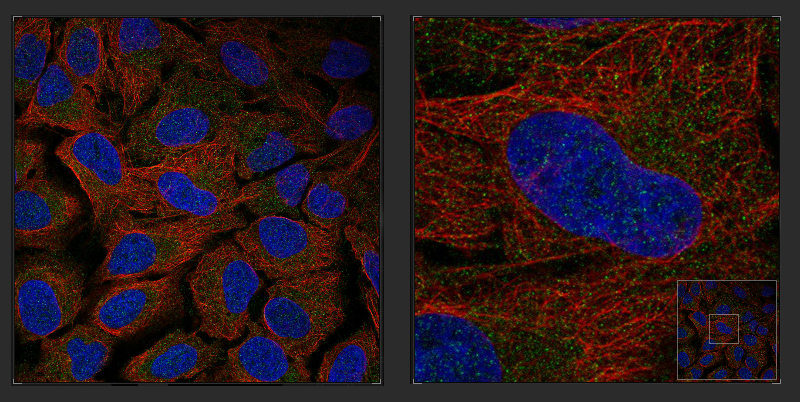
\includegraphics[scale=0.45]{zoom.png}}
	  \caption{\label{fig:zoom}An image with its original resolution and a zoomed in version. The mini-map in the bottom right corner of the zoomed in version shows the player the position of the zoom.}
	\end{figure}

	Below the image is a color channel filter which we implemented. It has four buttons which each gives a different version of the same image, with a different combination of red, green and blue although green is always present. Using the color channel filter can aid players in classifying images correctly as some patterns are more easily identified with certain filters.

	The player then compares the image with the 27 categories that are available. The categories are divided into four super categories, three of which cover different parts of the cell and one is for unidentifiable patterns. That way players can quickly see which super category they should be comparing with the image. The categories are laid out in a hexagonal pattern and each of them can be viewed more closely by hovering over it. Once the player identifies a category he feels matches the image he can select it by clicking it. An image can match up to six different categories although most images match one to three categories. When the player is satisfied that he has selected all the relevant categories he submits his classification by clicking the submit button. What follows then depends upon which phase of the game the player is currently at, we will discuss those phases later.

	Players get rewarded for submitting solutions to images based on their historical accuracy which we call an accuracy rating. The reason being that players would most likely be less motivated to play if the rewards were delayed and most of the time the solution to the task is unknown, so there is no way of knowing if a player's solution is correct or not when he submits it. Even if we sometimes know the correct answer to the task and can therefore reward players based on whether they got it right or not, we choose to always reward players based on their accuracy rating to keep the reward system consistent. Everyone begins with an accuracy rating of 50\% which then increases or decreases based on how well they perform. 

	\subsubsection{Tutorial}
		When a player opens up Project Discovery for the first time he must start by going through a tutorial phase. We created the tutorial from scratch with the exception of some tooltip functionality which was already in place, although we refined it. The purpose of the tutorial phase is to allow the player to familiarize himself with the controls and the user interface of the game as well as teaching him the basics of analyzing subcellular images. To achieve this we first introduce the player to the controls by using tooltips which explain the functionality of each control element, one at a time, while also allowing the player to interact with the controls. 

		%Tooltip screenshot
		\begin{figure}[H]
		  \centering
		  \graphicspath{ {./graphics/} }
		  \centerline{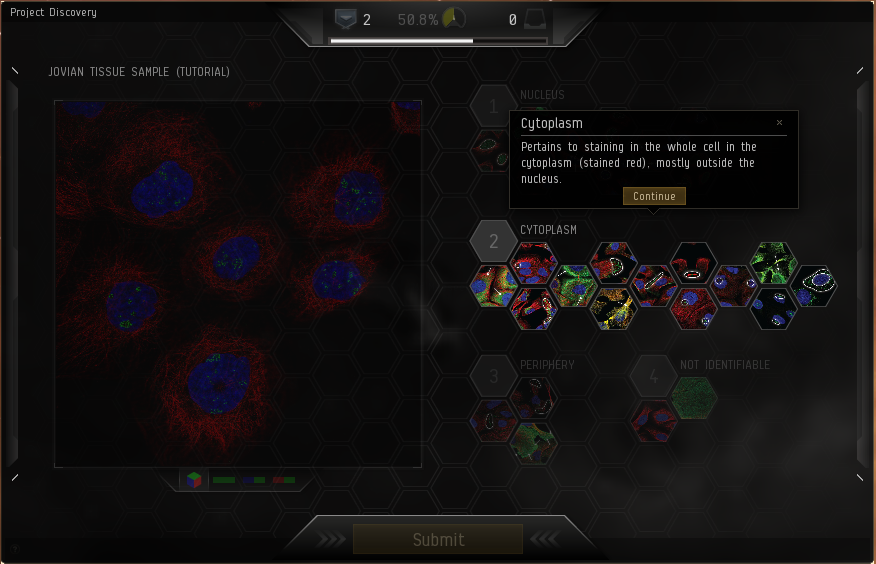
\includegraphics[scale=0.53]{tooltip.png}}
		  \caption{\label{fig:tooltip}The tooltip which explains the cytoplasm category, making it the only active part of interface.}
		\end{figure}

		Once the player has gone through the tooltips he gets his first image to analyze, this image is the first stage of seven in the tutorial. Each stage contains one image hand picked by scientists at the Human Protein Atlas and it presents a gradual increase in difficulty from the previous stage. To ease the player into the game and not overwhelm him with all 27 categories, we limit the number of categories available to choose from, to the correct ones plus a few similar but incorrect categories.

		%Limited categories screenshot
		\begin{figure}[H]
		  \centering
		  \graphicspath{ {./graphics/} }
		  \centerline{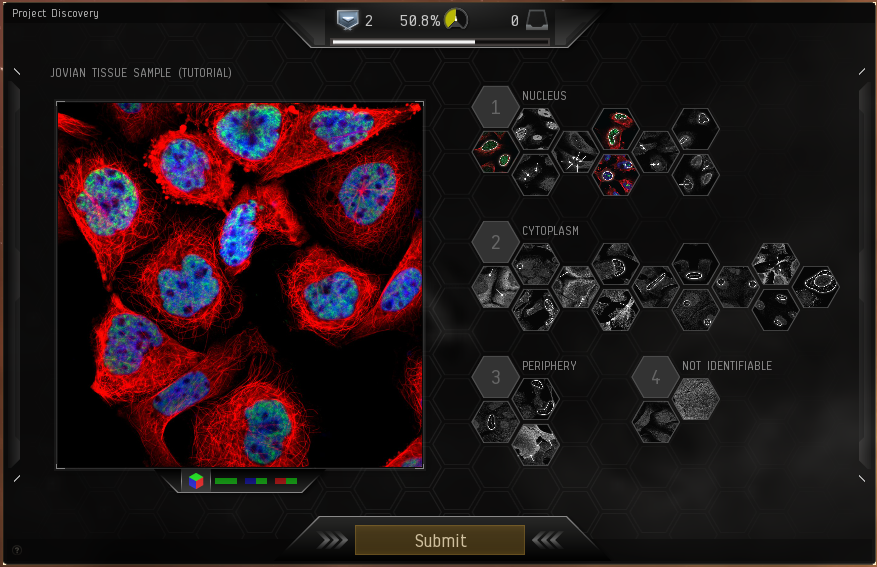
\includegraphics[scale=0.53]{limited.png}}
		  \caption{\label{fig:limited}An example of a tutorial stage where the categories are limited to only three nucleus categories.}
		\end{figure}

		When the player submits his classification a results screen is displayed. It shows the correct result by overlaying the categories the player picked with either a green correct or red incorrect texture and giving any categories that are correct but the player missed, a green outline texture indicating a missed category. By giving the player instant feedback on their submission we allow the player to learn from any possible mistakes they make. Players do not have to get the correct results for the seven stages of the tutorial to advance, we believed that could be a source of frustration since it would make the tutorial longer. 

		%Results screenshot
		\begin{figure}[H]
		  \centering
		  \graphicspath{ {./graphics/} }
		  \centerline{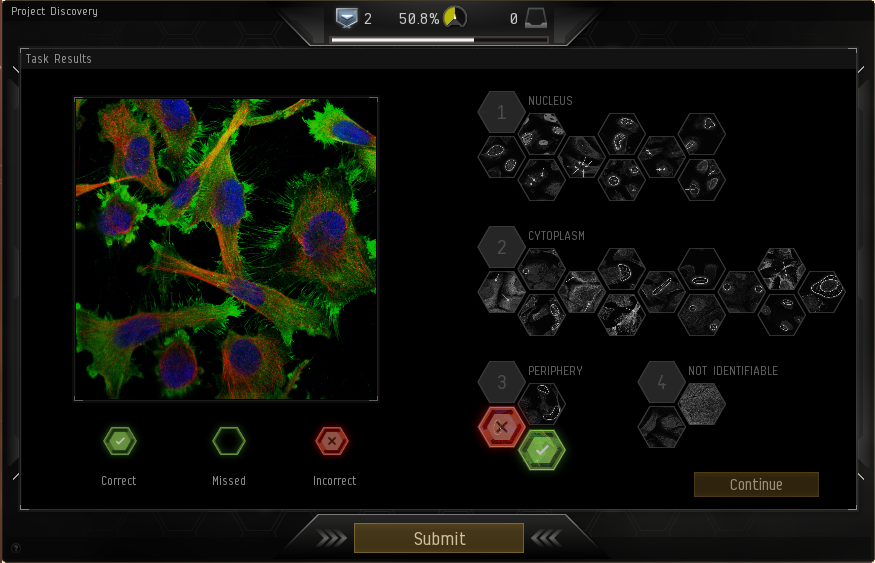
\includegraphics[scale=0.53]{result.png}}
		  \caption{\label{fig:result}The result screen which shows the player getting one category right and one wrong.}
		\end{figure}

	\subsubsection{Training tasks}
		After finishing the tutorial the player receives rewards for doing so and is then moved on to the next phase of the game which we refer to as the training phase. This phase, like the tutorial, consists of seven stages containing images that have already been classified by scientists. However, unlike the tutorial, players must get the correct result in each stage to advance to the next phase of the game. The stages also increase in difficulty and are in general more difficult than the tutorial images. Players get the same result screen as in the tutorial so they can continue to learn and better understand how to correctly classify images. 

		The purpose of this phase is to continue to teach players how to classify images and to make sure that only players that have the skills and/or will to solve images correctly can make it to the next phase and thereby contribute to classifying images that haven't already been classified by scientists. Since players get rewards for submitting solutions based on their accuracy rating, they can extract some amount of rewards even if they get everything wrong. We have to make arrangements for players who are only interested in getting rewards with as little effort as possible. With the training phase requiring players to get correct results to be able to move on to classify unknown images, those players would never get to that stage and therefore won't contaminate the results of those images. 

	\subsubsection{Unknown tasks}

\subsection{Network Communications}
	The Project Discovery client utilizes a connection with two different parts, the EVE server, and the MMOS RESTful API, which uses the Amazon CloudFront CDN and an Elastic Beanstalk container.

	% Útskýra af hverju þetta er POST en ekki GET
	When a player opens up the client, it automatically contacts the EVE server through a proxy provided by CCP because of security concerns. The server issues a POST request to the MMOS API through the proxy to ask for a new task for the player. The MMOS API then allocates a task for the specified player and fetches it from the Elastic Beanstalk container, which returns the appropriate task object to the EVE server, which finally sends it to the EVE client. 

	The task object includes a security pass that the client needs to access the URLs for each image that he needs for the task. Each time the client needs an image for that task, it contacts the EVE server, which contacts the MMOS API with the security pass. If that pass is still active, the Amazon CloudFront CDN returns a signed URL that leads to that image. As a security feature, the image itself is only accessible for a few seconds, so the client needs to cache the image in case the player needs to access it again. When a player has submitted his classification for the task, the EVE server issues a POST request to the MMOS API like before, and returns a solution or a community consensus that it uses to grade the player and which we can use to reward them in game.

	The MMOS API authentication uses a HMAC-SHA256 method, based on Amazon authentication methods. The server has an API key and secret, which are changed at regular intervals. The API key and secret are used to generate a signing key, this adds an additional layer of security, since every message is hashed with different values.

\subsection{Architecture}

	% Skrifað í stackless python, notast við UI library CCP, nefna klasana sem tilheyra leiknum, server kóðann

	The Project Discovery architecture follows EVE Online client architecture by example. The language used is Stackless Python, the code is located in a package within the EVE Online client, and contains a server side and a client side. The server side is split into two parts, the MMOS server and the Project Discovery server. 

	The Project Discovery server is used to contact the EVE database, to insert new players into tables and keeping track of their experience within Project Discovery. It also connects to the MMOS server, requesting tasks and their information, submitting classifications, and receiving player statistics. The MMOS server is the server that connects to the MMOS API through a CCP proxy. This server keeps the API keys and secrets, as well as allocating new authentication signatures each time a GET or POST request is made. This separation of the server side is necessary because of security reasons suggested by CCP employees.

	The Project Discovery client side mostly contains code for the user interface, which utilizes libraries already existing within the EVE Online codebase. The client side also contains all the logic for the tutorial, UI help, category tooltips, rewarding algorithm, animations, category exclusion, audio, scene switching, and the general handling of messages and information coming from the server side.

\subsection{The website}
	One of the goals of the project was to launch a Project Discovery website along with the release of the game. The website serves as an information hub for the project. Interested parties can get information about the game, the science behind the game and our partners, MMOS and the Human Protein Atlas. The website also displays videos related to the game and screenshots of the game in action. To build the website we used HTML5, Less and JavaScript. We were provided with a template from web developers within CCP which helped us make the website look professional and consistent with other EVE Online websites.

	%Setja inn mynd af vefsíðu? Yeb